\section{Rovfugle (vildtkending og biologi)}

\begin{frame}
  \vspace{1.5em}
  \begin{center}
    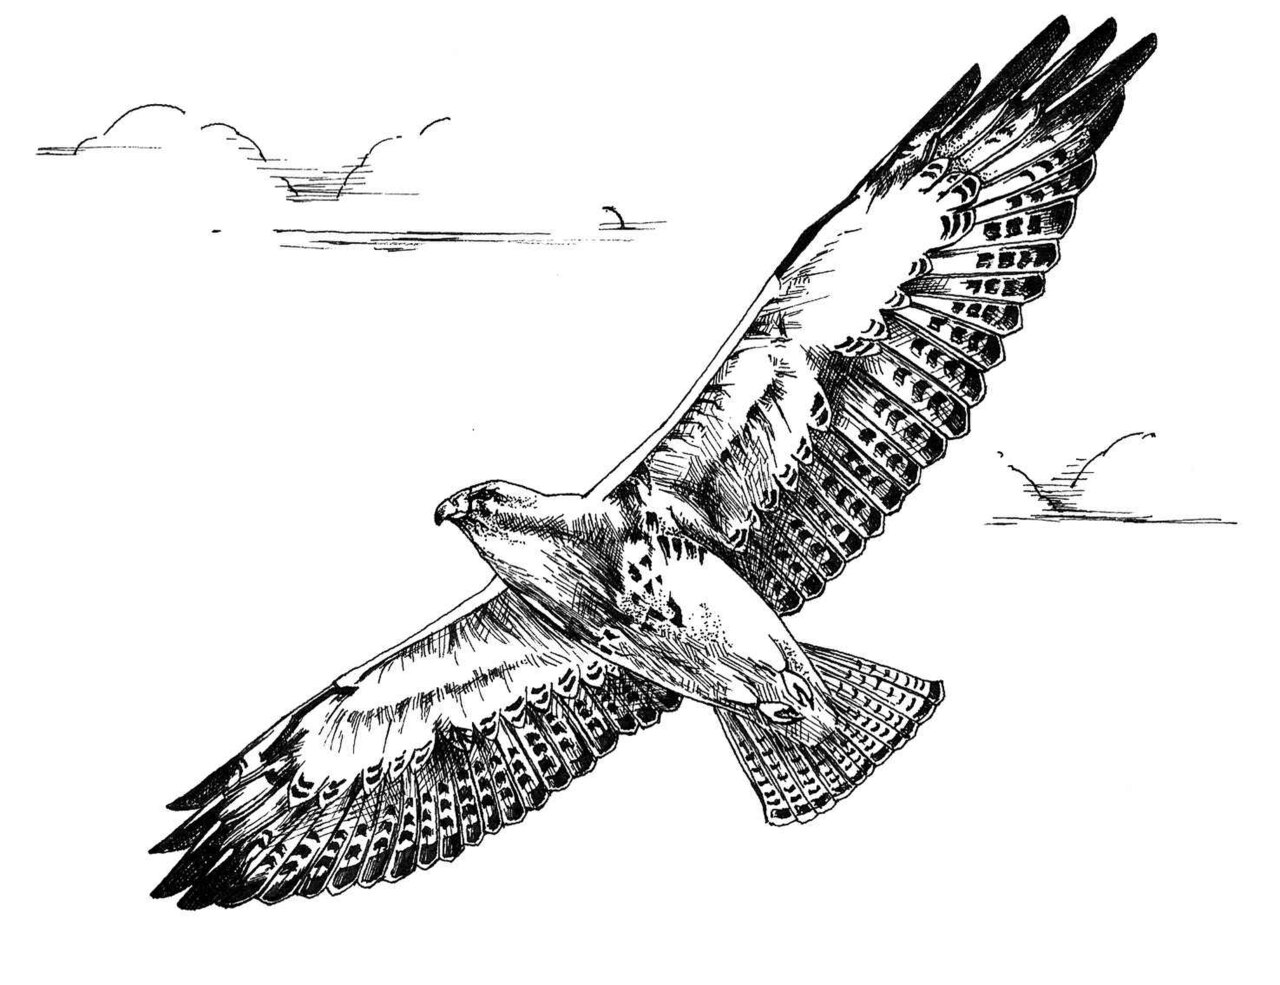
\includegraphics[width=12cm, height=4cm, keepaspectratio]{Billeder/Dyr/Fugle/Rovfugle/rovfugle.jpg}\\[1.2em]
    {\LARGE \textbf{Rovfugle}}
    \vspace{1em}
    \\ Artsbestemmelse og vildtbiologi
    \\[0.9em]
    {\tiny\color{gray}
    CC BY 4.0 – kan frit anvendes, også kommercielt. Rettighederne må ikke skærpes.\\[0.05em]
    Udviklet af Aleksander Sønder, OSJAGTTEGN.DK}
  \end{center}
\end{frame}

% ========== MUSVÅGE ==========
\begin{frame}{%
  \begin{minipage}[c]{0.30\textwidth}
    Musvåge
  \end{minipage}%
  \hfill
  \begin{minipage}[c]{0.45\textwidth}
    \footnotesize
    \textbf{Jagttid:} Ingen jagttid
  \end{minipage}%
  \hfill
  \begin{minipage}[c]{0.15\textwidth}
    \noindent\raggedleft
    
\includegraphics[width=0.5cm, height=0.5cm, keepaspectratio]{Billeder/Ikoner/star.png}%
    \hspace{0.2em}%
    
\includegraphics[width=0.5cm, height=0.5cm, keepaspectratio]{Billeder/Ikoner/star.png}
  \end{minipage}%
}
  \vspace{0.25em}
  \begin{columns}[T]
    % --- Venstre kolonne: Tekst ---
    \column{0.45\textwidth}
    \setlength{\parskip}{0.5em}
    \tiny
    \RaggedRight
    \textbf{\textit{Buteo buteo}} – kraftig bredskuldret rovfugl med musende kald \par
    \textbf{Udseende:}\\
    \quad – Brun men kan variere fra mørk til lys. Spraglet bryst. \par
    \textbf{Levesteder:} Det åbne land. \par
    \textbf{Føde:} Mus, gnavere, orme, frøer, harekillinger. \par
    \textbf{Udbredelse:} Hele Danmark. \par
    \textbf{Træk/standfugl:} Begge
    % --- Højre kolonne: Større billede ---
    \column{0.52\textwidth}
    \centering
    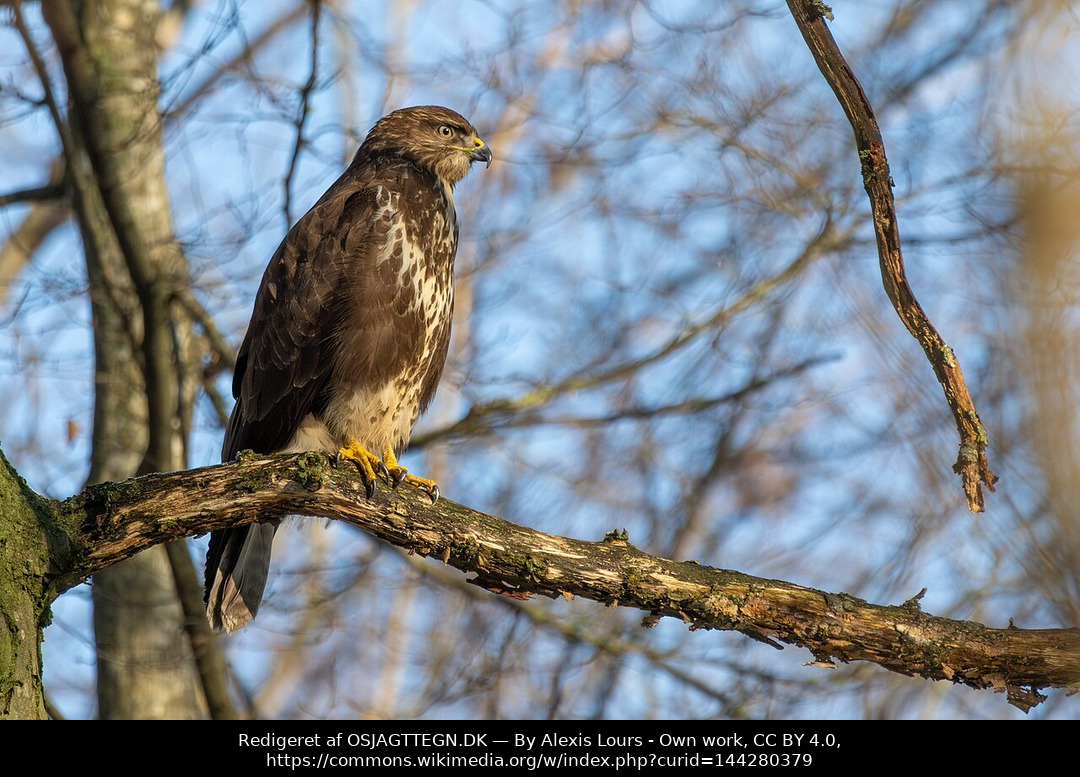
\includegraphics[width=\linewidth, height=7.2cm, keepaspectratio]{Billeder/Dyr/Fugle/Rovfugle/musvåge.jpg}
  \end{columns}
\end{frame}
% ========== SPURVEHØG ==========
\begin{frame}{%
  \begin{minipage}[c]{0.30\textwidth}
    Spurvehøg
  \end{minipage}%
  \hfill
  \begin{minipage}[c]{0.45\textwidth}
    \footnotesize
    \textbf{Jagttid:} Ingen jagttid
  \end{minipage}%
  \hfill
  \begin{minipage}[c]{0.15\textwidth}
    \noindent\raggedleft
    
\includegraphics[width=0.5cm, height=0.5cm, keepaspectratio]{Billeder/Ikoner/star.png}%
    \hspace{0.2em}%
    
\includegraphics[width=0.5cm, height=0.5cm, keepaspectratio]{Billeder/Ikoner/star.png}
  \end{minipage}%
}
  \vspace{0.25em}
  \begin{columns}[T]
    % --- Venstre kolonne: Tekst ---
    \column{0.45\textwidth}
    \setlength{\parskip}{0.5em}
    \tiny
    \RaggedRight
    \textbf{\textit{Accipiter nisus}} – relativt lille rovfugl \par
    \textbf{Udseende:}\\
    \quad – Tynde gule tændstiksben, rustrøde tværstriber på bryst \par
    \textbf{Levesteder:} Skovområder men forefindes også i byområder. \par
    \textbf{Føde:} Spurve og drosler som fanges ved overraskelse. \par
    \textbf{Udbredelse:} Hele Danmark. \par
    \textbf{Træk/standfugl:} Begge
    % --- Højre kolonne: Større billede ---
    \column{0.52\textwidth}
    \centering
    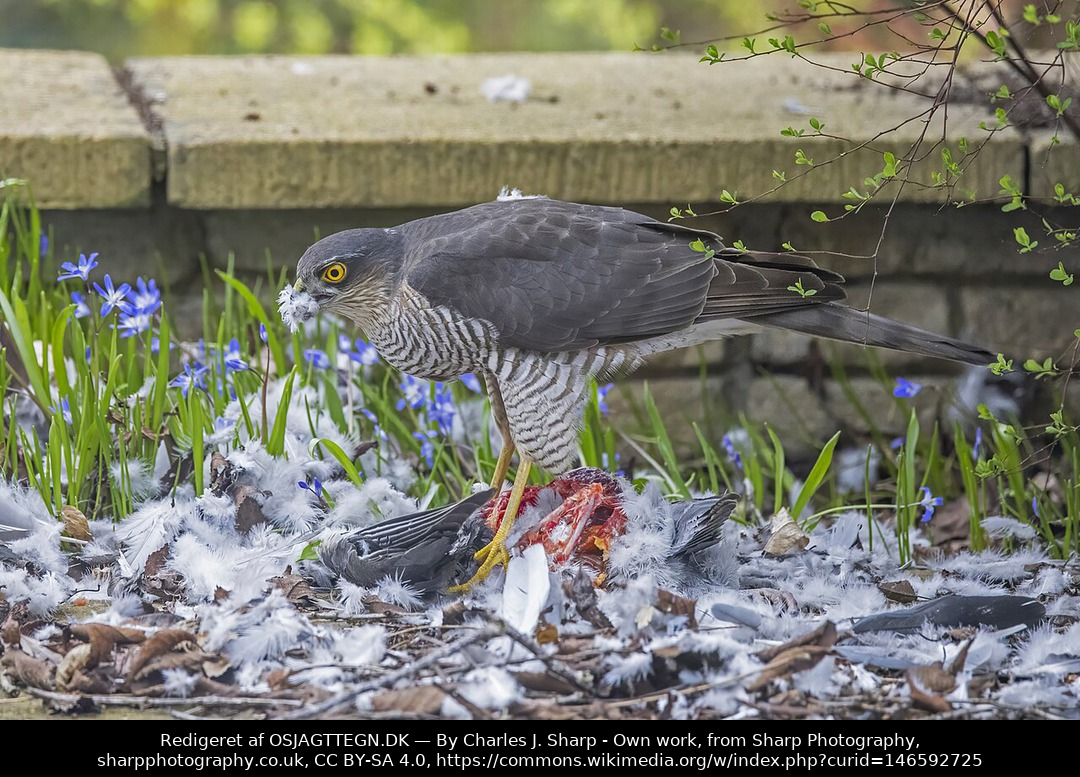
\includegraphics[width=\linewidth, height=7.2cm, keepaspectratio]{Billeder/Dyr/Fugle/Rovfugle/spurvehøg.jpg}
  \end{columns}
\end{frame}
% ========== TÅRNFALK ==========
\begin{frame}{%
  \begin{minipage}[c]{0.30\textwidth}
    Tårnfalk
  \end{minipage}%
  \hfill
  \begin{minipage}[c]{0.45\textwidth}
    \footnotesize
    \textbf{Jagttid:} Ingen jagttid
  \end{minipage}%
  \hfill
  \begin{minipage}[c]{0.15\textwidth}
    \noindent\raggedleft
    
\includegraphics[width=0.5cm, height=0.5cm, keepaspectratio]{Billeder/Ikoner/star.png}%
    \hspace{0.2em}%
    
\includegraphics[width=0.5cm, height=0.5cm, keepaspectratio]{Billeder/Ikoner/star.png}
  \end{minipage}%
}
  \vspace{0.25em}
  \begin{columns}[T]
    % --- Venstre kolonne: Tekst ---
    \column{0.45\textwidth}
    \setlength{\parskip}{0.5em}
    \tiny
    \RaggedRight
    \textbf{\textit{Falco tinnunculus}} – en af de mest udbredte rovfugle i Danmark \par
    \textbf{Udseende:}\\
    \quad – Teglrød overside med pletter, mørke tværbånd på halen \par
    \textbf{Levesteder:} Åbne arealer, også i byer og langs veje. \par
    \textbf{Føde:} Mus, gnavere og insekter. \par
    \textbf{Udbredelse:} Hele Danmark. \par
    \textbf{Træk/standfugl:} Begge
    % --- Højre kolonne: Større billede ---
    \column{0.52\textwidth}
    \centering
    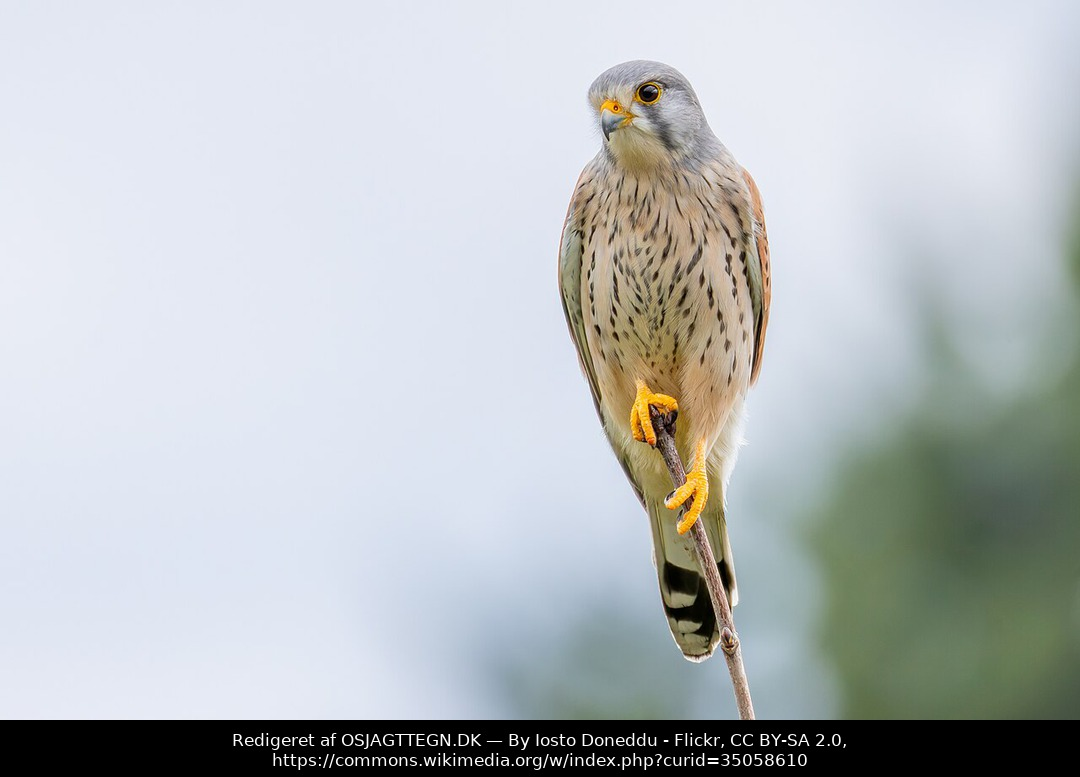
\includegraphics[width=\linewidth, height=7.2cm, keepaspectratio]{Billeder/Dyr/Fugle/Rovfugle/tårnfalk.jpg}
  \end{columns}
\end{frame}
% ========== DUEHØG ==========
\begin{frame}{%
  \begin{minipage}[c]{0.30\textwidth}
    Duehøg
  \end{minipage}%
  \hfill
  \begin{minipage}[c]{0.45\textwidth}
    \footnotesize
    \textbf{Jagttid:} Ingen jagttid
  \end{minipage}%
  \hfill
  \begin{minipage}[c]{0.15\textwidth}
    \noindent\raggedleft
    
\includegraphics[width=0.5cm, height=0.5cm, keepaspectratio]{Billeder/Ikoner/star.png}
  \end{minipage}%
}
  \vspace{0.25em}
  \begin{columns}[T]
    % --- Venstre kolonne: Tekst ---
    \column{0.45\textwidth}
    \setlength{\parskip}{0.5em}
    \tiny
    \RaggedRight
    \textbf{\textit{Accipiter gentilis}} – stor høg \par
    \textbf{Udseende:}\\
    \quad – Grå, med tværtstriber på bryst, lys øjenstribe
    % --- Højre kolonne: Større billede ---
    \column{0.52\textwidth}
    \centering
    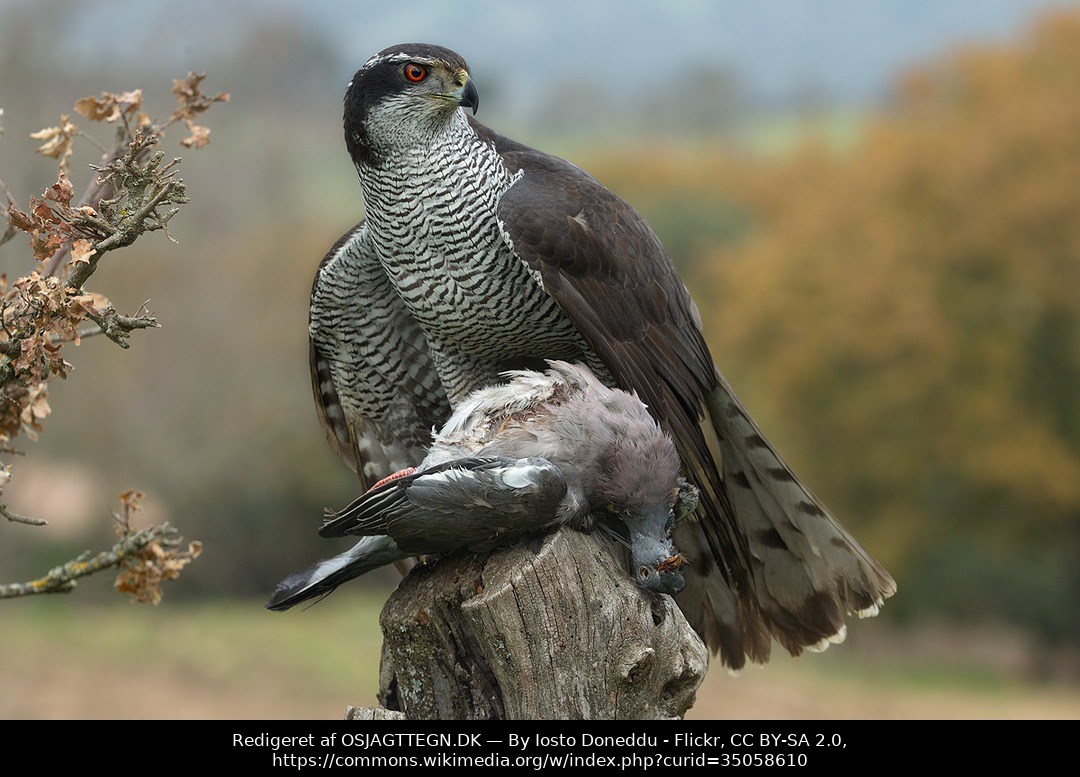
\includegraphics[width=\linewidth, height=7.2cm, keepaspectratio]{Billeder/Dyr/Fugle/Rovfugle/duehoeg.jpg}
  \end{columns}
\end{frame}
% ========== VANDREFALK ==========
\begin{frame}{%
  \begin{minipage}[c]{0.30\textwidth}
    Vandrefalk
  \end{minipage}%
  \hfill
  \begin{minipage}[c]{0.45\textwidth}
    \footnotesize
    \textbf{Jagttid:} Ingen jagttid
  \end{minipage}%
  \hfill
  \begin{minipage}[c]{0.15\textwidth}
    \noindent\raggedleft
    
\includegraphics[width=0.5cm, height=0.5cm, keepaspectratio]{Billeder/Ikoner/star.png}
  \end{minipage}%
}
  \vspace{0.25em}
  \begin{columns}[T]
    % --- Venstre kolonne: Tekst ---
    \column{0.45\textwidth}
    \setlength{\parskip}{0.5em}
    \tiny
    \RaggedRight
    \textbf{\textit{Falco peregrinus}} – mellemstor falk – kan flyve 150 km/t \par
    \textbf{Udseende:}\\
    \quad – Tynde tværstriber med sort pilothjelm. Bemærk skægstriben
    % --- Højre kolonne: Større billede ---
    \column{0.52\textwidth}
    \centering
    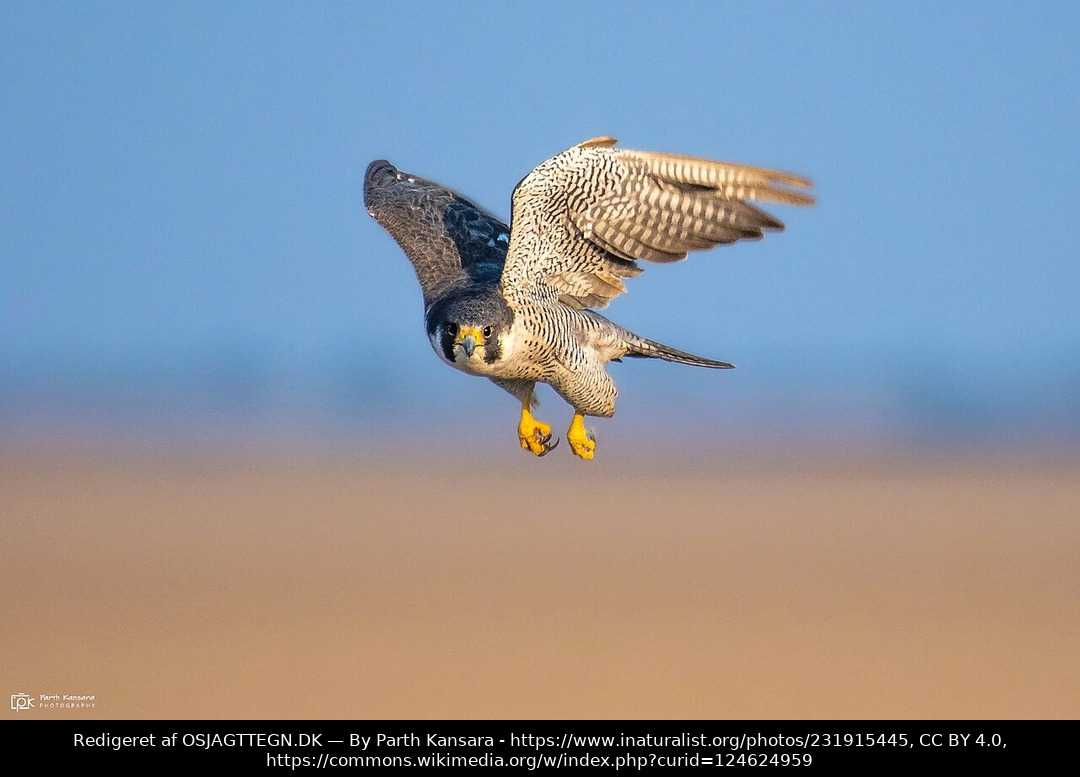
\includegraphics[width=\linewidth, height=7.2cm, keepaspectratio]{Billeder/Dyr/Fugle/Rovfugle/vandrefalk.jpg}
  \end{columns}
\end{frame}
% ========== RØRHØG ==========
\begin{frame}{%
  \begin{minipage}[c]{0.30\textwidth}
    Rørhøg
  \end{minipage}%
  \hfill
  \begin{minipage}[c]{0.45\textwidth}
    \footnotesize
    \textbf{Jagttid:} Ingen jagttid
  \end{minipage}%
  \hfill
  \begin{minipage}[c]{0.15\textwidth}
    \noindent\raggedleft
    
\includegraphics[width=0.5cm, height=0.5cm, keepaspectratio]{Billeder/Ikoner/star.png}
  \end{minipage}%
}
  \vspace{0.25em}
  \begin{columns}[T]
    % --- Venstre kolonne: Tekst ---
    \column{0.45\textwidth}
    \setlength{\parskip}{0.5em}
    \tiny
    \RaggedRight
    \textbf{\textit{Circus aeruginosus}} – i familien kærhøge som er kendetegnet ved v-formen i vingerne \par
    \textbf{Udseende:}\\
    \quad – Flødegult hovede og bryst, lange ben
    % --- Højre kolonne: Større billede ---
    \column{0.52\textwidth}
    \centering
    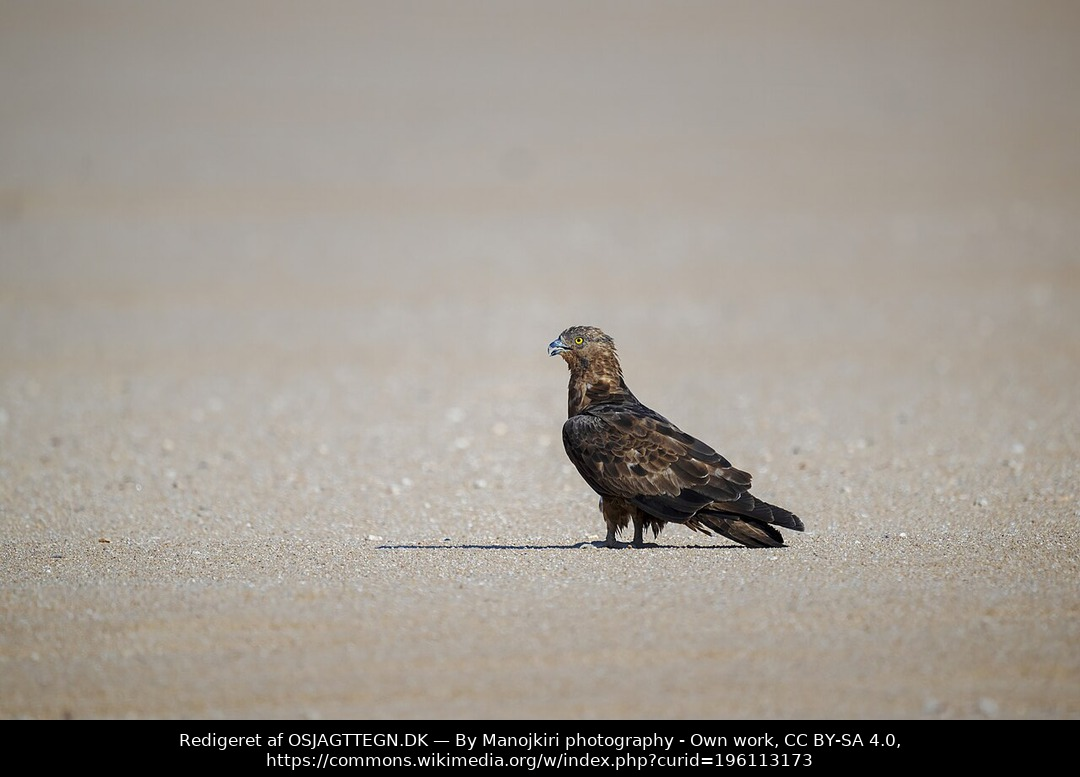
\includegraphics[width=\linewidth, height=7.2cm, keepaspectratio]{Billeder/Dyr/Fugle/Rovfugle/rørhøg.jpg}
  \end{columns}
\end{frame}
% ========== FISKEØRN ==========
\begin{frame}{%
  \begin{minipage}[c]{0.30\textwidth}
    Fiskeørn
  \end{minipage}%
  \hfill
  \begin{minipage}[c]{0.45\textwidth}
    \footnotesize
    \textbf{Jagttid:} Ingen jagttid
  \end{minipage}%
  \hfill
  \begin{minipage}[c]{0.15\textwidth}
    \noindent\raggedleft
    
\includegraphics[width=0.5cm, height=0.5cm, keepaspectratio]{Billeder/Ikoner/star.png}
  \end{minipage}%
}
  \vspace{0.25em}
  \begin{columns}[T]
    % --- Venstre kolonne: Tekst ---
    \column{0.45\textwidth}
    \setlength{\parskip}{0.5em}
    \tiny
    \RaggedRight
    \textbf{\textit{Pandion haliaetus}} – mellemstor rovfugl med lange smalle vinger \par
    \textbf{Udseende:}\\
    \quad – Grå overside, hvid underside. Hvidt hoved med sort stribe langsgående med halsen. Blå ben
    % --- Højre kolonne: Større billede ---
    \column{0.52\textwidth}
    \centering
    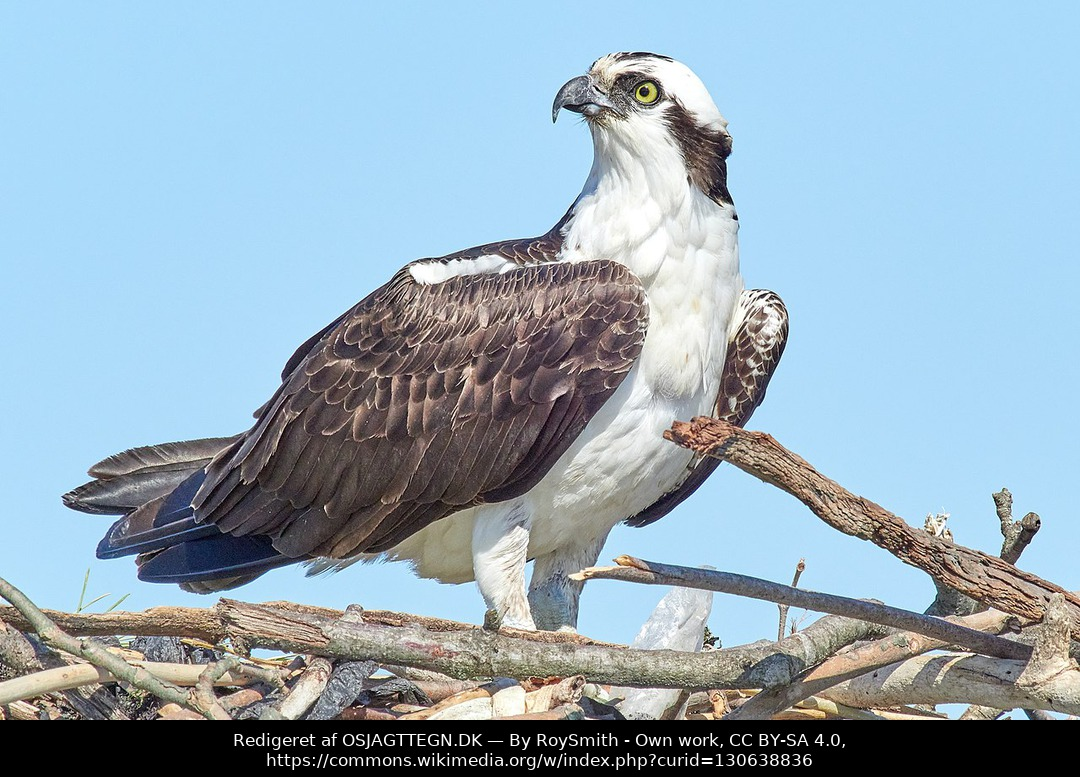
\includegraphics[width=\linewidth, height=7.2cm, keepaspectratio]{Billeder/Dyr/Fugle/Rovfugle/fiskeørn.jpg}
  \end{columns}
\end{frame}